	\subsection{La méthode Scrum}
	\begin{frame}{\large Scrum, une méthodologie de développement}
		\only<2>{
		\vspace{15px}
		}
		\begin{block}{Scrum : méthode agile}
			\begin{itemize}
				\item Incrémental
				\item Absence d'effet tunnel
			\end{itemize}
			\begin{figure}[H]
				\centering
				\vspace{-15px}
				\only<2>{
				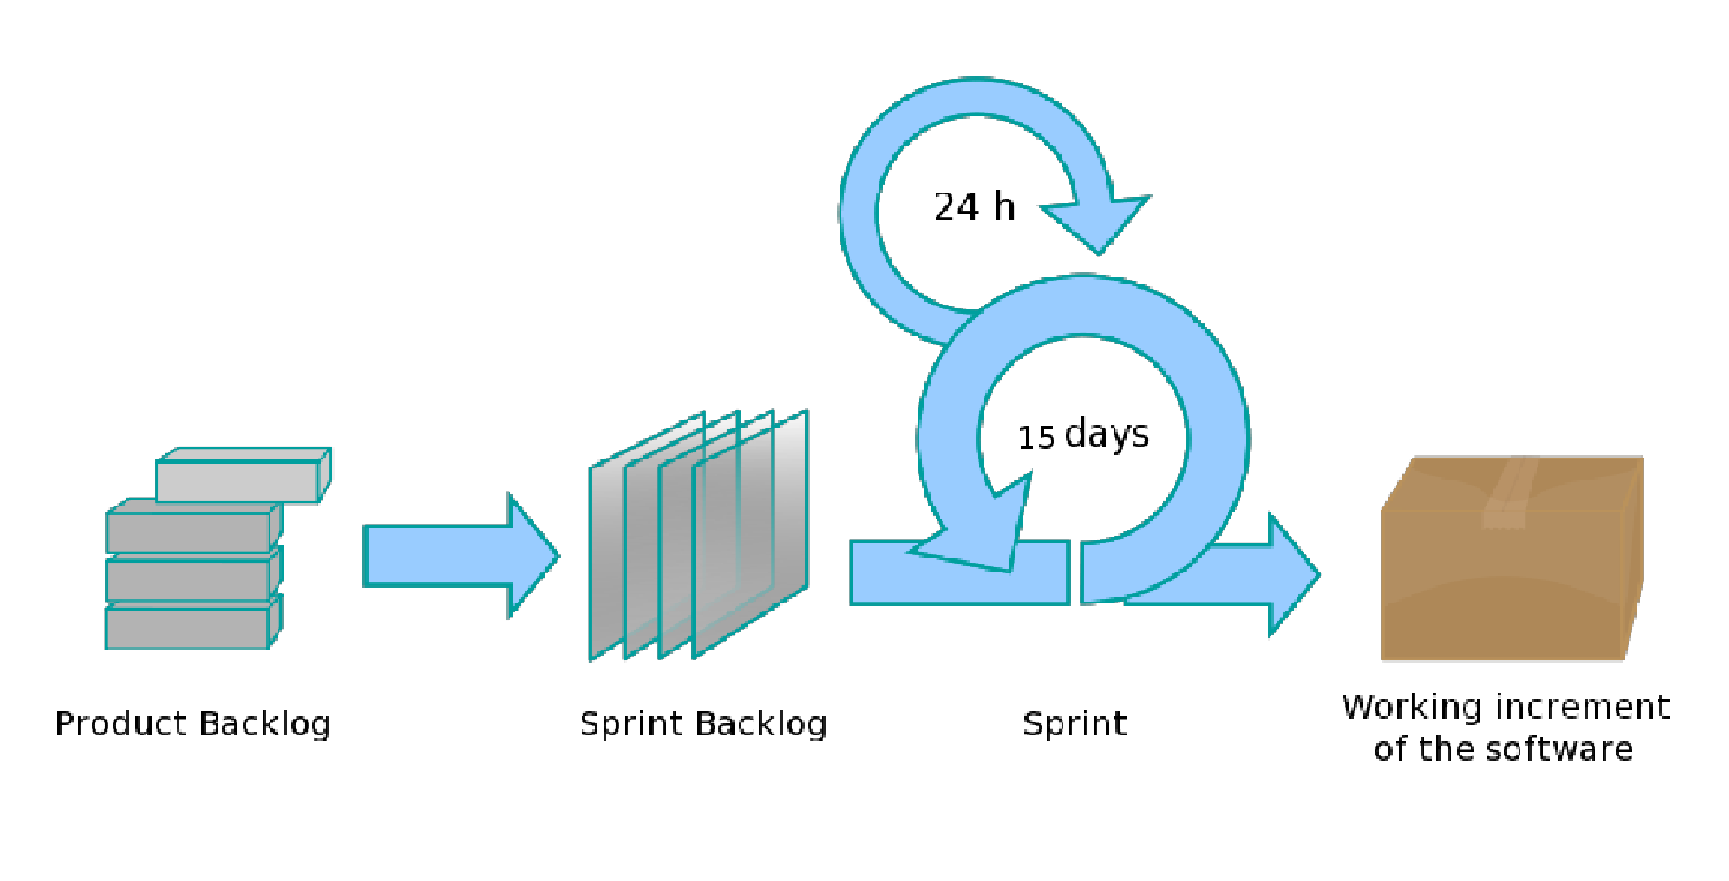
\includegraphics[width=5.8cm]{images/Scrum_process.eps}
				}
				\only<3->{
				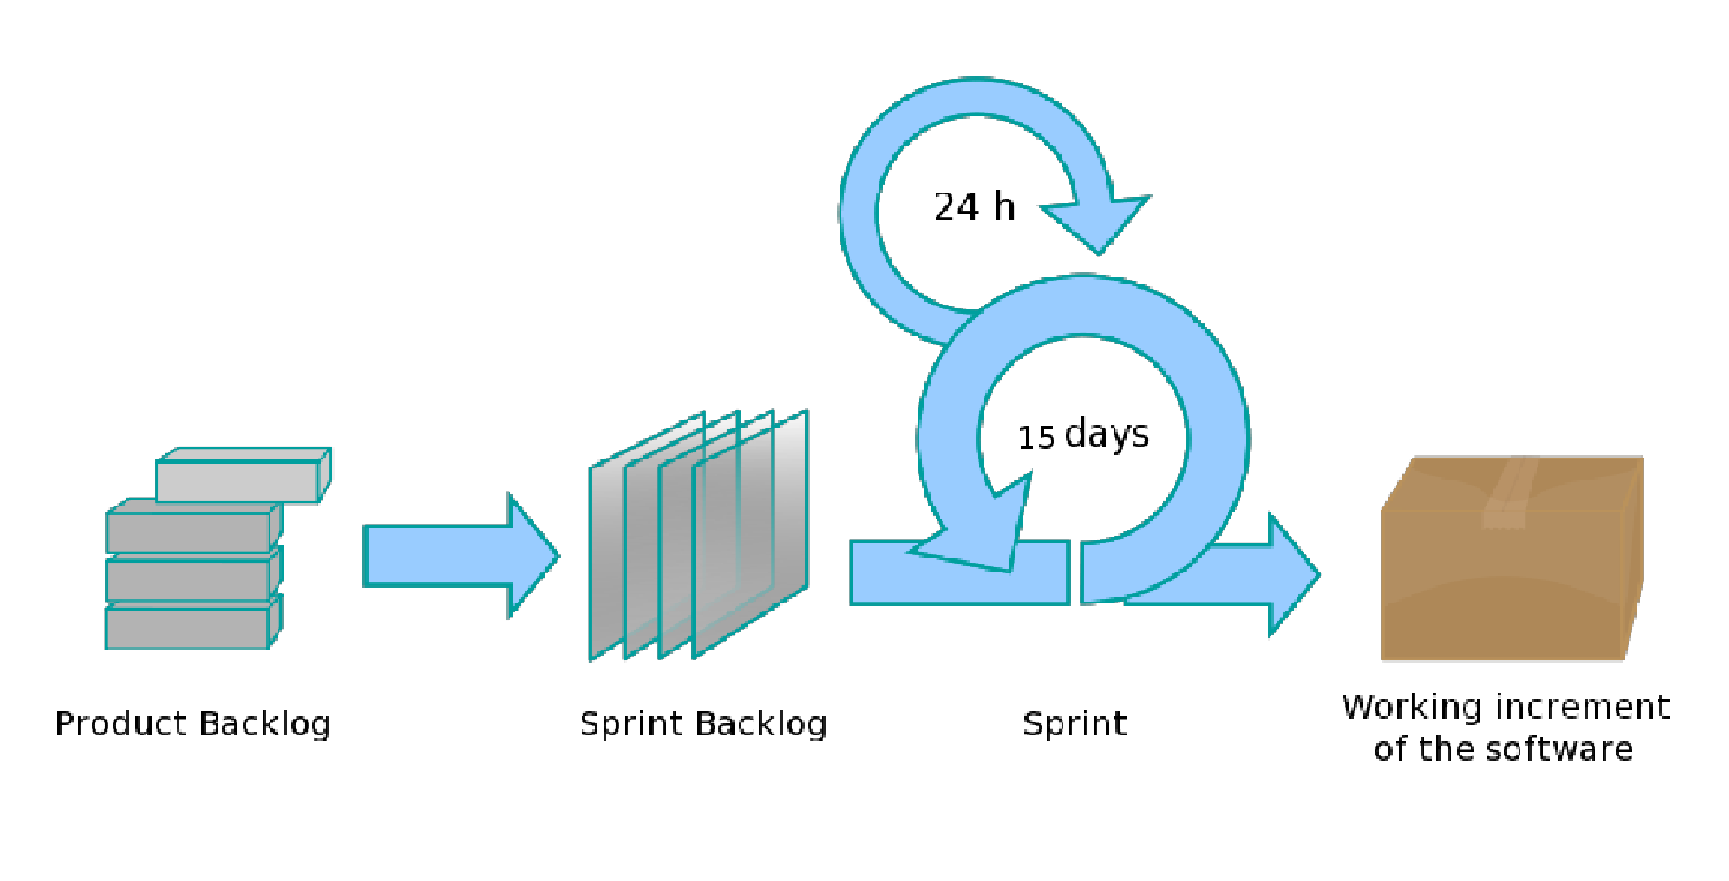
\includegraphics[width=2.8cm]{images/Scrum_process.eps}
				}
				\only<2->{
				\vspace{-10px}
				\caption{Processus de développement Scrum}
				}
			\end{figure}
		\end{block}
		\uncover<3->{
		\begin{block}{User Stories}
			\begin{itemize}
				\item Fonctionnalités
				\item Finie
					\begin{itemize}
						\item 
\includegraphics[height=7px]{images/coverage.png}~~Couverture de code > 80\% % TODO image
						\item 
\includegraphics[height=7px]{images/build.png}~~Build passing % TODO image 
						\item \texttt{// Code documenté}
						\item 
\includegraphics[height=9px]{images/pullrequest.png}~~Code relu et validé par une tierce personne
					\end{itemize}
			\end{itemize}
		\end{block}
		}
	\end{frame}
	\begin{frame}{\large Scrum, une méthodologie de développement}
		\begin{block}{Organisation}
			\begin{tabular}{cc}
				\begin{minipage}{0.36\textwidth}
					\setbeamercovered{transparent}{
					\begin{itemize}
						\item<1,4-> Backlog
						\item<2,4-> Planning Poker
						\item<3,4-> Mêlées
					\end{itemize}
					}
				\end{minipage}&
				\begin{minipage}{0.6\textwidth}
					\begin{figure}[H]
						\only<1>{
						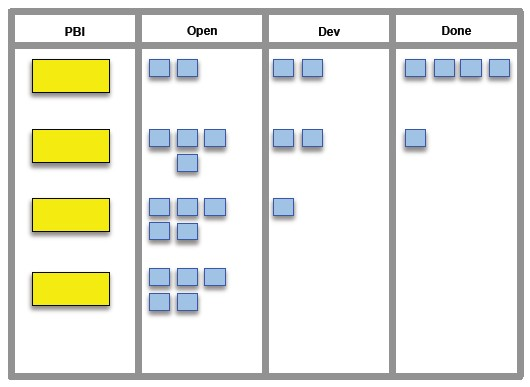
\includegraphics[height=2.5cm]{images/backlog.jpg}
						}
						\only<2>{
						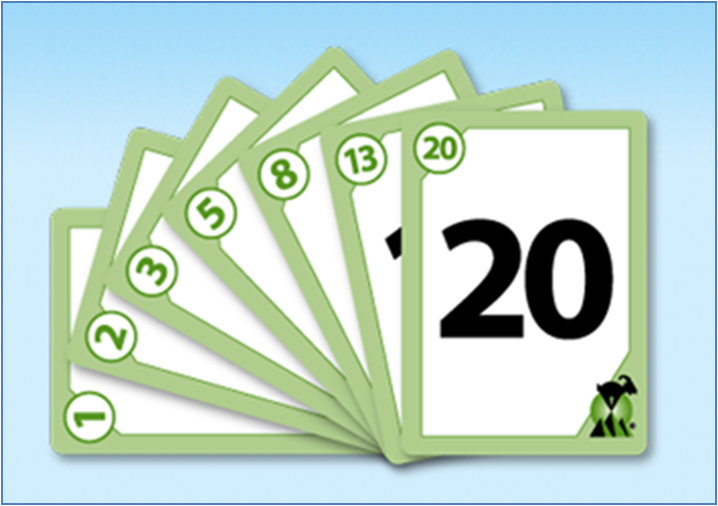
\includegraphics[height=2.5cm]{images/cards-planning-poker.png}
						}
						\only<3>{
						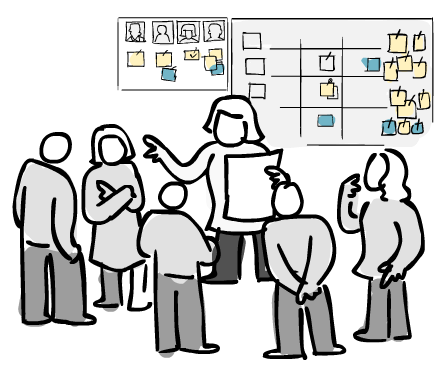
\includegraphics[height=2.5cm]{images/melees.png}
						}
						\only<4->{
						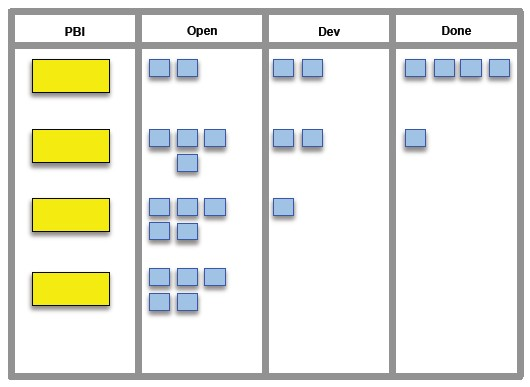
\includegraphics[height=1.2cm]{images/backlog.jpg}~
						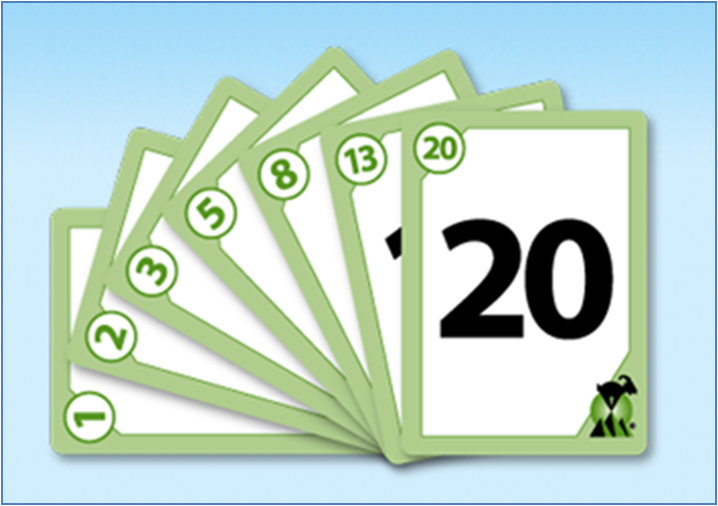
\includegraphics[height=1.2cm]{images/cards-planning-poker.png}~
						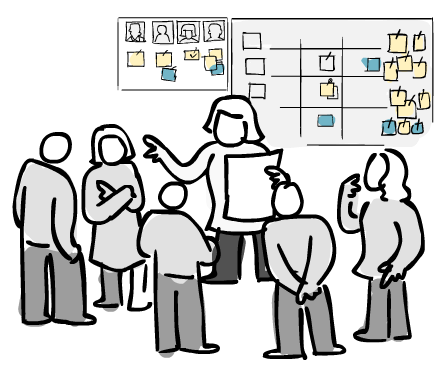
\includegraphics[height=1.2cm]{images/melees.png}
						}
					\end{figure}
				\end{minipage}
			\end{tabular}
		\end{block}
		\uncover<4->{
		\begin{block}{Les différents rôles}
			\begin{tabular}{cc}
				\begin{minipage}{0.36\textwidth}
					\setbeamercovered{transparent}{
					\begin{itemize}
						\item<5> Scrum Master
						\item<6> Product Owner
						\item<7> Responsable technique
						\item<8> Équipe de développement
					\end{itemize}
					}
				\end{minipage}&
				\begin{minipage}{0.6\textwidth}
					\begin{figure}[H]
						\centering
						\only<5>{
						
\includegraphics[height=2.5cm]{images/photos/kratux.png}
						}
						\only<6-7>{
						
\includegraphics[height=2.5cm]{images/photos/satenske.png}
						}
						\only<8>{
						
\includegraphics[height=1.5cm]{images/photos/kratux.png}~
						
\includegraphics[height=1.5cm]{images/photos/satenske.png}\newline
						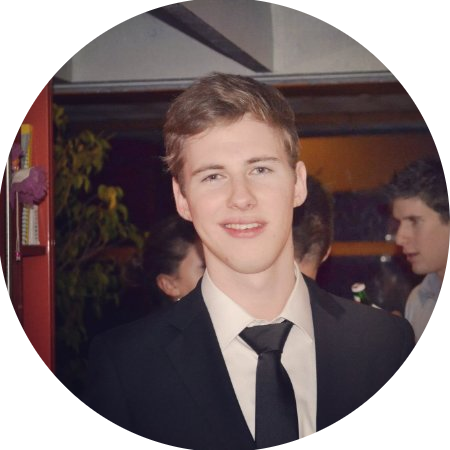
\includegraphics[height=1.5cm]{images/photos/oxynos.png}~
						
\includegraphics[height=1.5cm]{images/photos/tsoo.png}
						}
					\end{figure}
				\end{minipage}
			\end{tabular}
		\end{block}
		}
	\end{frame}
	% Pull Requests	
	% Branching flow
	\subsection{L'intégration continue}
	\begin{frame}{Intégration\ldots}
		\begin{block}{Git et Github}
			\begin{tabular}{cc}
				\begin{minipage}{0.5\textwidth}
					\begin{itemize}
							\uncover<1->{
						\item Contrôle de version 
						\item Fusion automatique
							}
							\uncover<2->{
						\item Communication
						\item Issues
							}
					\end{itemize}
				\end{minipage} & 
				\begin{minipage}{0.48\textwidth}
					\begin{figure}[H]
						\hspace{-49px}
						\uncover<1->{
						\vspace{25px}
						
\includegraphics[height=1.6cm]{logos/gitvertical.png}~
						}
						\uncover<2->{
						
\includegraphics[height=1.6cm]{logos/githubvertical.png}
						}
					\end{figure}
				\end{minipage}
			\end{tabular}
		\end{block}
	\end{frame}
	\begin{frame}{Intégration\ldots}
		\begin{figure}[H]
			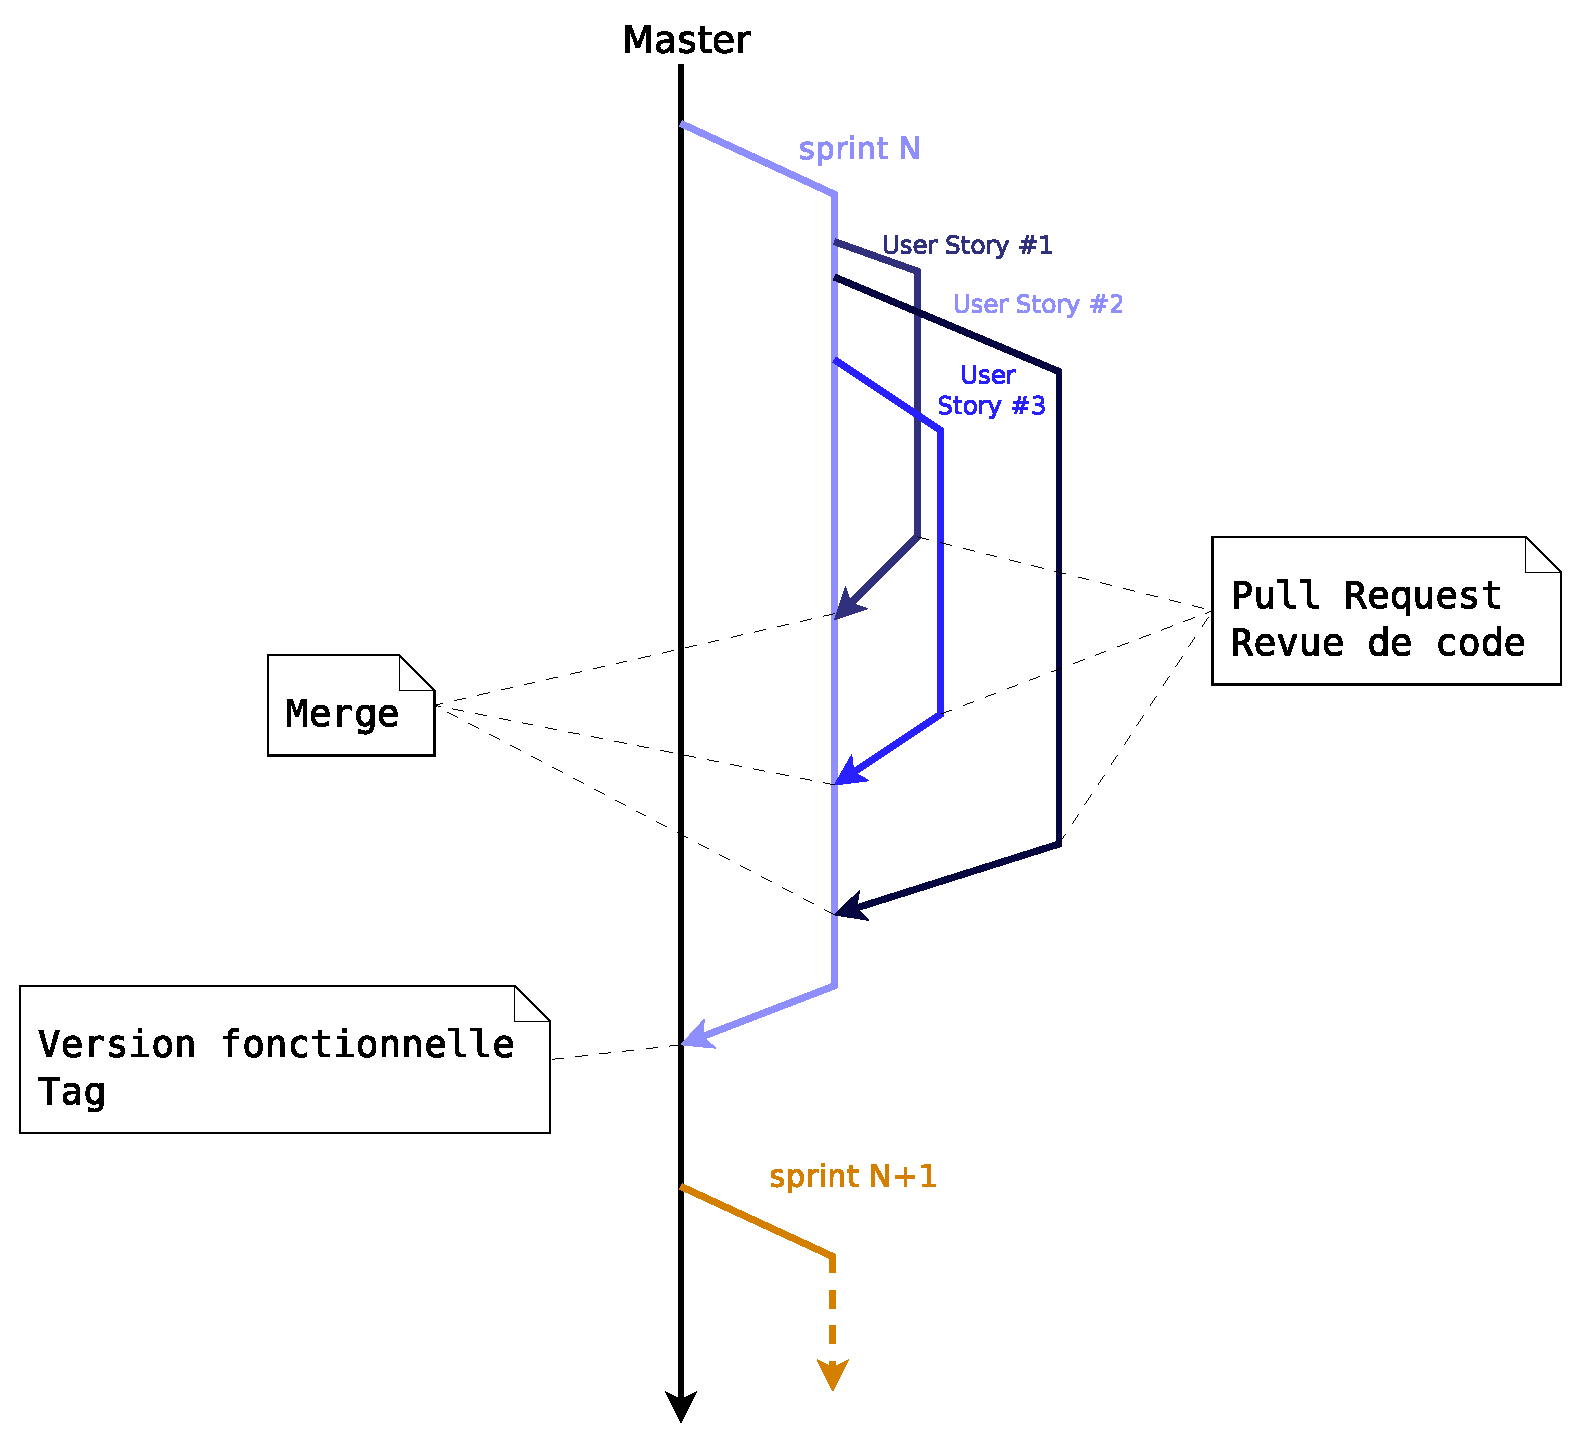
\includegraphics[height=7.5cm]{images/BranchingWorkflow.eps}
			\vspace{-10px}
			\caption{Git Branching}
		\end{figure}
	\end{frame}

	\begin{frame}{\ldots Continue}
		\begin{figure}[H]
			\centering
			\only<1>{
			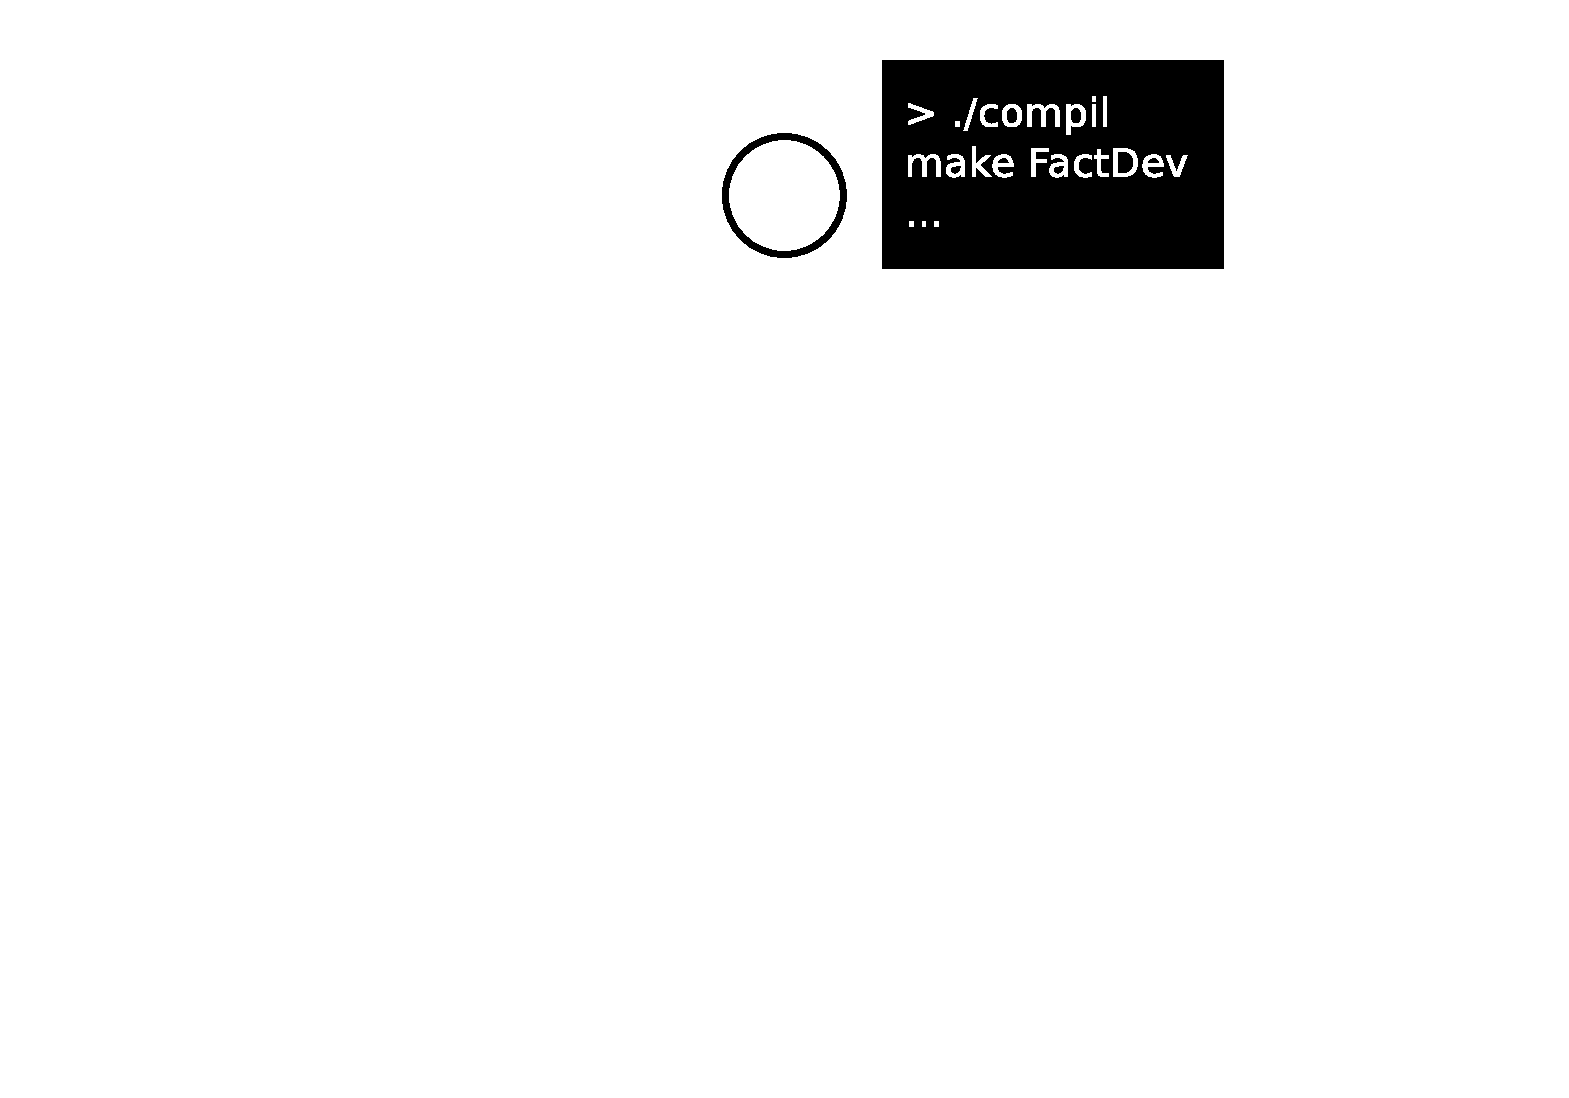
\includegraphics[width=9cm]{images/Travis/travis1_compil.eps}
			}
			\only<2>{
			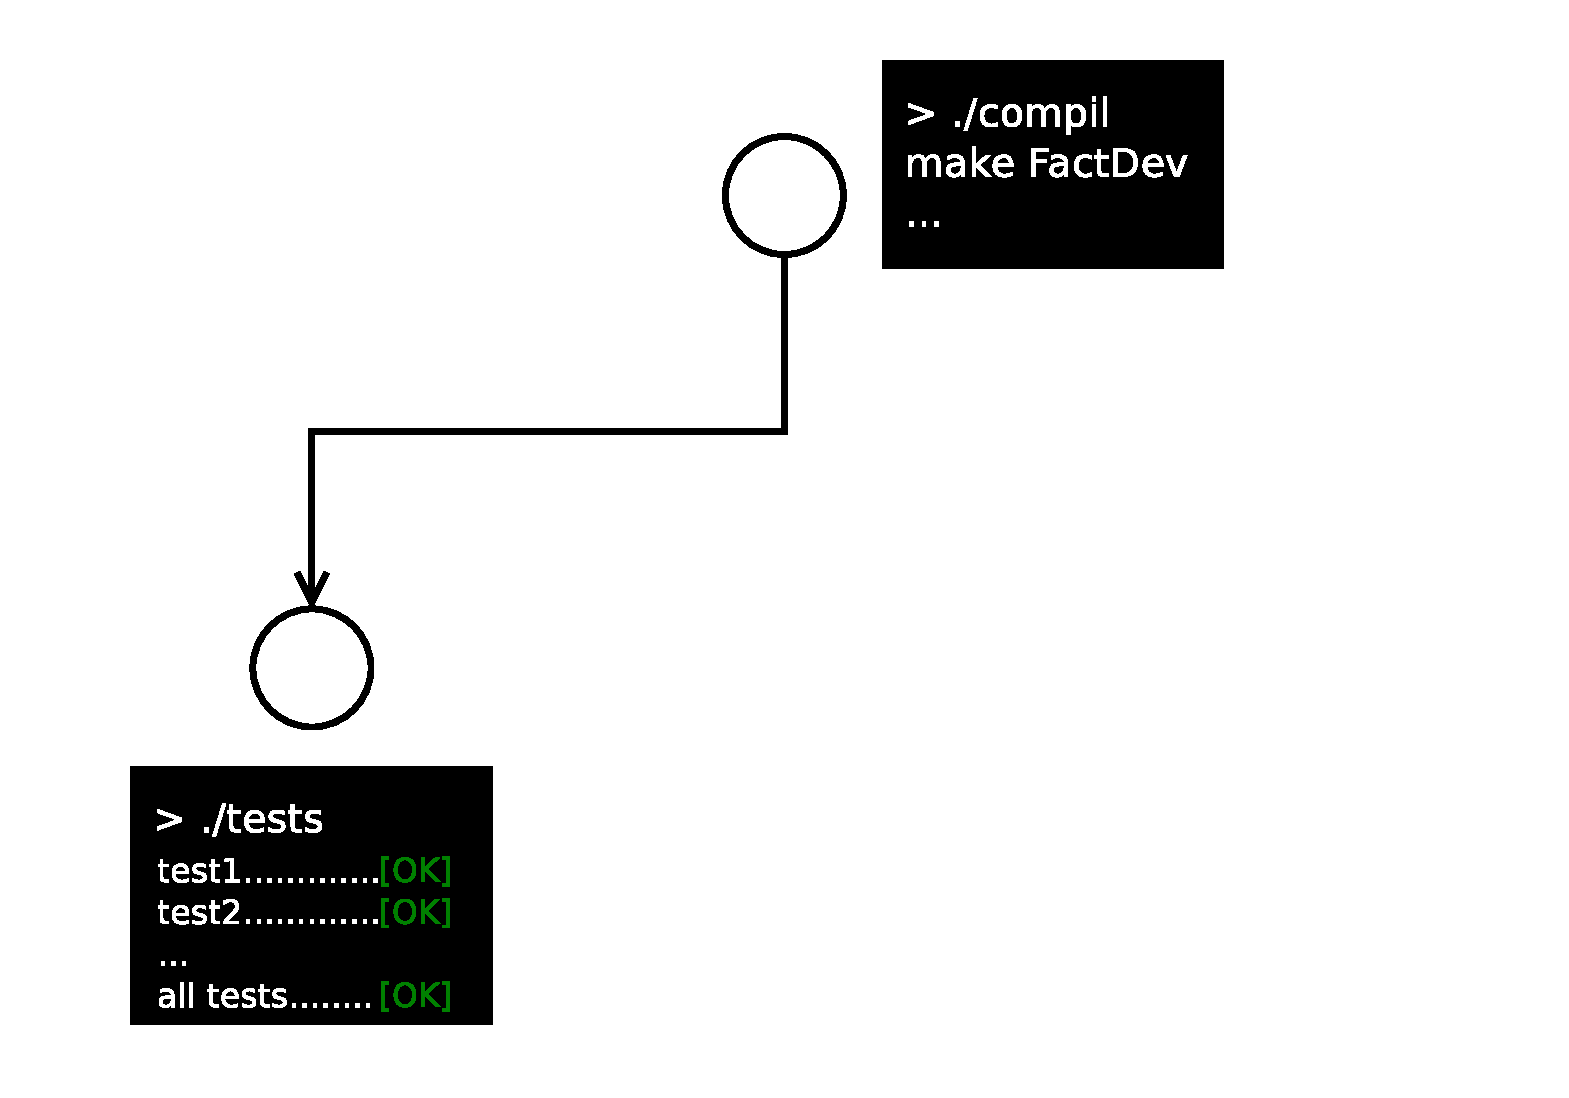
\includegraphics[width=9cm]{images/Travis/travis2_tests.eps}
			}		
			\only<3>{
			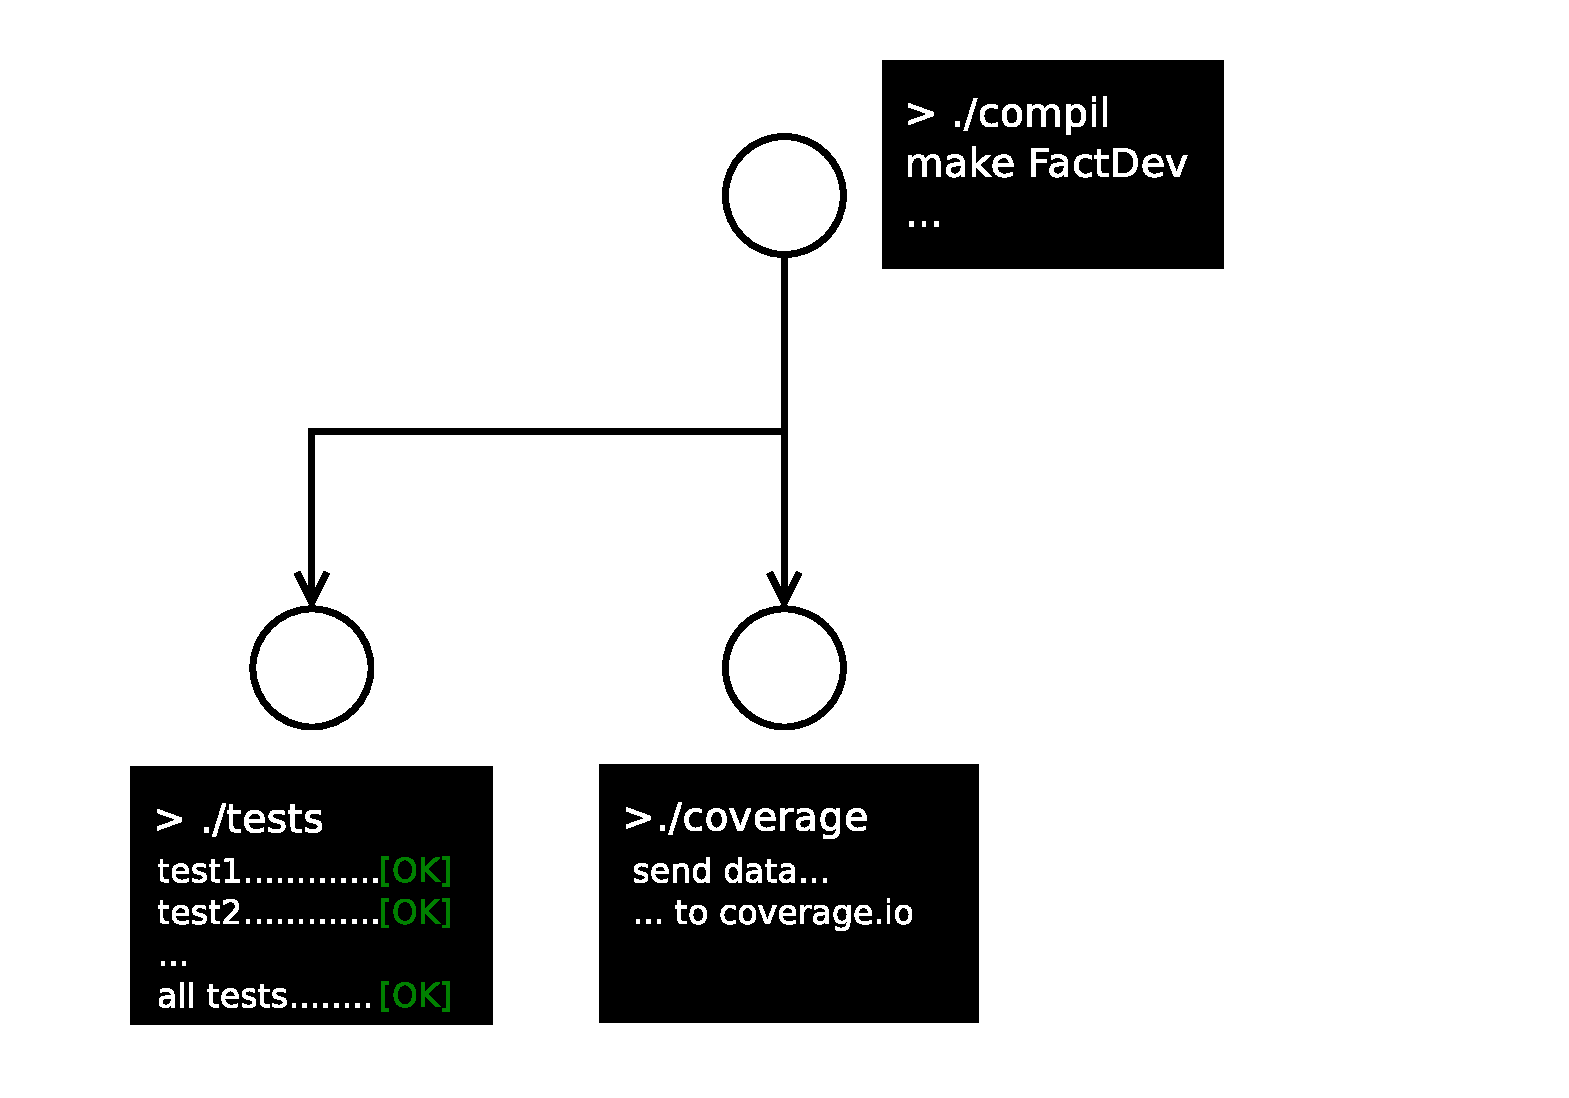
\includegraphics[width=9cm]{images/Travis/travis3_coverage.eps}
			}	
			\only<4>{
			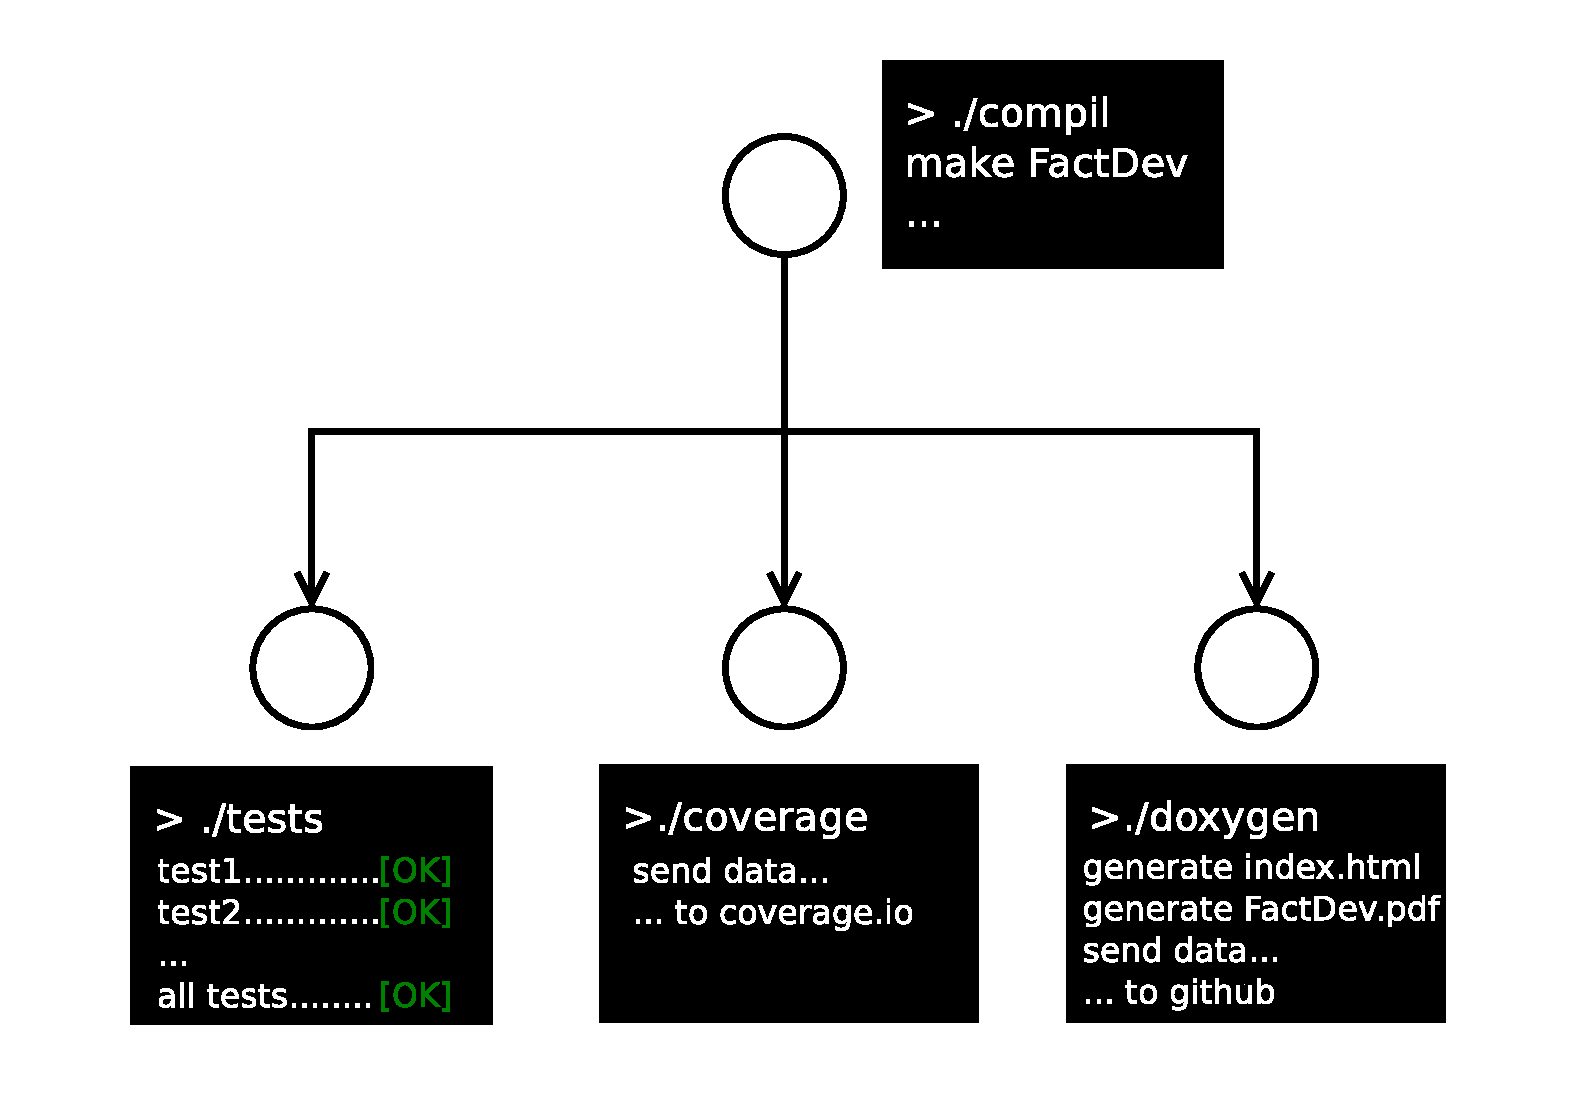
\includegraphics[width=9cm]{images/Travis/travis4_doxygen.eps}
			\newline 
			
\includegraphics[height=8px]{images/build.png} 
			}	
			\only<5>{
			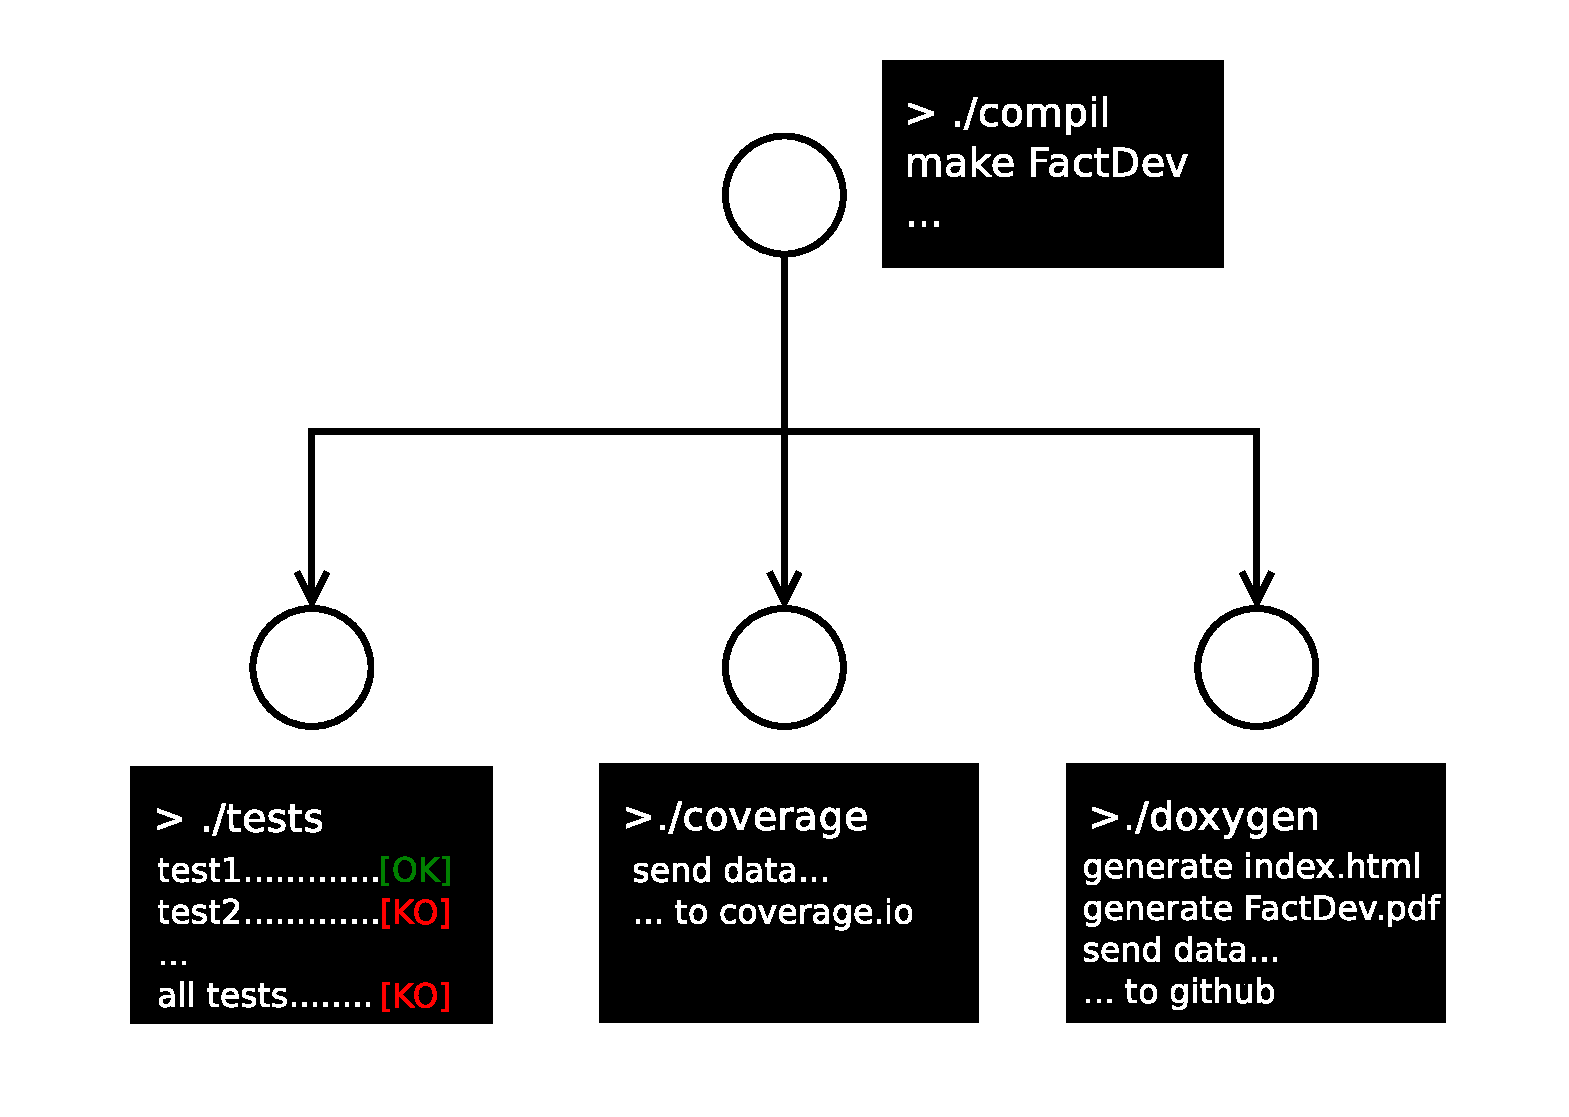
\includegraphics[width=9cm]{images/Travis/travis5_fail.eps}
			\newline 
			
\includegraphics[height=8px]{images/build_failing.png} 
			}

			\caption{Intégration continue avec Travis CI}
		\end{figure}

		% Couverture de code
		% Build, 
		% Tests
		% Transition vers la revue de code :)

		\end{frame}
		\subsection{La revue de code}
		\begin{frame}{Vers 100\% de revue de code}
			\begin{itemize}
				\item Toutes intégrations nécessitent une \textbf{Pull Request}
			\end{itemize}
			\vfill
			\pause
			\begin{block}{\normalsize Validation d'une Pull Request par une tierce personne}
				\begin{itemize}
					\item Le code
						\begin{itemize}
							\item Est lisible
							\item Est compréhensible
							\item Respecte les conventions d'écriture
						\end{itemize}
					\item Les tests fonctionnels sont validés
					\item Le code est documenté
					\item 
\includegraphics[height=7px]{images/all_is_well.png}
						\begin{itemize}
							\item Le build passe
							\item Pas de régression de la couverture de code
						\end{itemize}
				\end{itemize}
			\end{block}	
		\end{frame}
